\documentclass[11pt]{article}
%\usepackage{fullpage}
%\usepackage[margin=0.1in]{geometry}
\usepackage{amsfonts, amsthm, amssymb, amsmath}
%\usepackage[lined,boxed,commentsnumbered]{algorithm2e}
\usepackage[pdftex]{graphicx,color}
\usepackage[scaled=0.92]{helvet}
%\usepackage{times}
\usepackage[pdftex, pagebackref=true, colorlinks=true, urlcolor=blue, citecolor=blue, linkcolor=blue]{hyperref}
\usepackage{framed}
\usepackage{verbatim}
\usepackage{fullpage}
\usepackage{epsfig}
\linespread{0.94}

\def\ShowAuthNotes{1}
\def\alb{\allowbreak}
\addtolength{\textheight} {2.2cm}
\addtolength{\textwidth} {0.5cm}
% Theorem environments

\newtheorem{thm}{Theorem}[section]
\newtheorem{lem}[thm]{Lemma}
\newtheorem{cor}[thm]{Corollary}
\newtheorem{defn}[thm]{Definition}
\newtheorem{clm}[thm]{Claim}
\newtheorem{cons}[thm]{Construction}
\newtheorem{prop}[thm]{Proposition}
\newtheorem{problem}[thm]{Problem}

\newenvironment{theorem}{\begin{thm}\begin{rm}}%
    {\end{rm}\end{thm}}
\newenvironment{lemma}{\begin{lem}\begin{rm}}%
    {\end{rm}\end{lem}}
\newenvironment{corollary}{\begin{cor}\begin{rm}}%
    {\end{rm}\end{cor}}
\newenvironment{definition}{\begin{defn}\begin{em}}%
    {\end{em}\end{defn}}
\newenvironment{claim}{\begin{clm}\begin{rm}}%
    {\end{rm}\end{clm}}
\newenvironment{construction}{\begin{cons}\begin{em}}%
    {\end{em}\end{cons}}
\newenvironment{proposition}{\begin{prop}\begin{em}}%
    {\end{em}\end{prop}}

\newcommand{\secref}[1]{\hyperref[#1]{Section \ref{#1}}}
\newcommand{\apref}[1]{\hyperref[#1]{Appendix \ref{#1}}}
\newcommand{\thref}[1]{\hyperref[#1]{Theorem \ref{#1}}}
\newcommand{\defref}[1]{\hyperref[#1]{Definition \ref{#1}}}
\newcommand{\corref}[1]{\hyperref[#1]{Corollary \ref{#1}}}
\newcommand{\lemref}[1]{\hyperref[#1]{Lemma \ref{#1}}}
\newcommand{\clref}[1]{\hyperref[#1]{Claim \ref{#1}}}
\newcommand{\consref}[1]{\hyperref[#1]{Construction \ref{#1}}}
\newcommand{\figref}[1]{\hyperref[#1]{Figure \ref{#1}}}
\newcommand{\eqnref}[1]{\hyperref[#1]{Equation \ref{#1}}}

\newcommand{\Prob}[1]{\Pr\left[\: #1 \:\right]}
\newcommand{\Adv}{\mathbf{Adv}}
\newcommand{\Exp}{\mathbf{Exp}}

\newcommand{\AdvOW}[2]{\Adv^{\mathrm{ow}}_{#1}(#2)}
\newcommand{\AdvAOW}[2]{\Adv^{\mathrm{aow}}_{#1}(#2)}

\def\gets{\leftarrow}
\def\getsr{\stackrel{\$}{\leftarrow}}

% \newcommand{\heading}[1]{{\vspace{6pt}\noindent\sc{#1}}}
% \newcommand{\vectornorm}[1]{\left|\left|#1\right|\right|}
% \newcommand{\ds}{\displaystyle}
\newcommand{\TODO}[1]{${\bf{\textcolor{red}{**** \text{#1} ****}}}$}

\begin{comment}
  \author{Some random fellow\vspace{-2ex}% Toggle commenting out the command
  }
  \date{A long time ago}
  \title{A comprehensive treatise on everything\vspace{-2ex}% to see the effect
  }
\end{comment}

% \begin{comment}
\title{{\bf{\vspace{-8ex}Algorithms for Vehicle Routing}}
}
\vspace{0.01in}
\author{
Kyle Davis\footnote{CS Undergraduate Student, College of Computing, Georgia Institute of Technology. Email : {\em{kdavis@gatech.edu}}} \ and Daniel Hull\footnote{CS Undergraduate Student, College of Computing, Georgia Institute of Technology. Email : {\em{dhull6@gatech.edu}}} \\
  Mentors: Henrik I. Christensen\footnote{School of Interactive Computing, Georgia Institute of Technology, Atlanta, GA-30332.} \ and Prasad Tetali\footnote{School of Mathematics and School of Computer Science, Georgia Institute of Technology, Atlanta, GA-30332.}
}
\date{}
% \end{comment}
\begin{document}
% \vspace*{-1cm}
\pagestyle{empty}
\maketitle
\thispagestyle{empty}
\vspace*{-1cm}
% \newpage
%%%%%%%%%%%%%%%%%%%%%%%%% 

% \begin{abstract}
%   Write something here.
% \end{abstract}

\section{Introduction}

Vehicle routing has been a challenging problem since the advent of self driving vehicles and robots. This problem is interesting due to its wide range of applications. Vehicle routing algorithms can be used to route packages through large networks, analyze and help improve traffic patterns, and be used to improve the efficiency of shipping warehouses. Working with several shipping companies we have tailored our algorithms to achieve the best performance under the last application. Everything from topology of the warehouse, distribution of the jobs, ordering of the jobs, and the vehicle routes influence the efficiency a warehouse can achieve.

\section{Problem Statement}

Given a topology and a list of packages, move the packages from their source to destination while minimizing the total duration. A topology is a 2-D grid containing sources, destinations, and vehicles. Vehicles are not allowed to collide with other vehicles, sources or destinations. Sources are black, destinations are red, and vehicles are red or blue circles depending on if they are currently carrying a package. The figures below represent two different topologies with the vehicles in the process of running their respective routes. \\

\TODO{Use 2 different topologies here}

\begin{center}
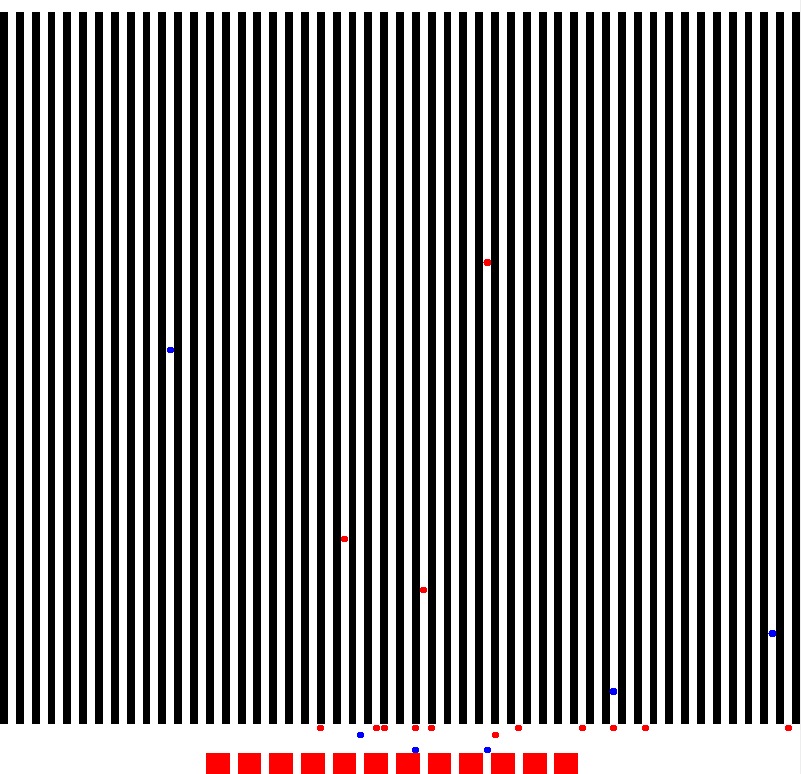
\includegraphics[height=200px]{topo_1.png} \ \ \ 
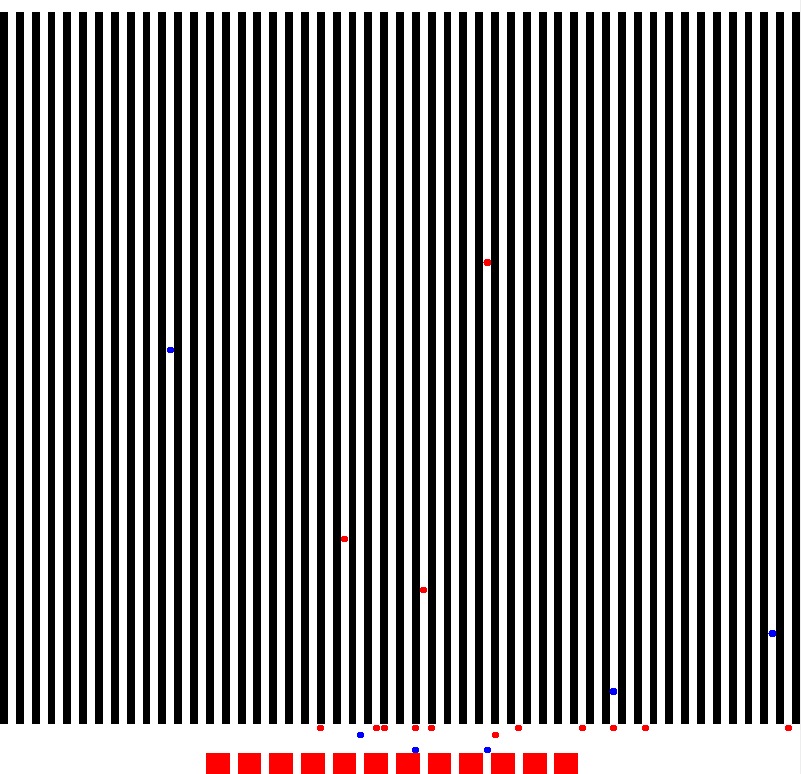
\includegraphics[height=200px]{topo_2.png}
\end{center}

The list of packages is given in a specific order and describes the source each package is originally located at, and the destination it must travel to. Usually there is a partial ordering that must be maintained when delivering packages, the packages must arrive in the order given as input to each destination. The problem has been relaxed to ignore the ordering restriction as well as allowing the vehicles to have infinite acceleration. This means that vehicles can accelerate to their maximum (unit) velocity and deccelerate to zero velocity instantaneously.

\section{Solution Strategies}

There were many aspects to this problem. Our initial research was focused on determining which parts of the problem had the greatest impact on overall effeciency. This will pave the way to more focused research related to the most important parts of vehicle routing. With a goal of implementing these solutions and improving the performance of warehouses around the world.

\subsection{Topology}

When desigining a toplogy there is a tradeoff beween space and speed. With more space vehicles have more room and avoiding collisions becomes easier allowing for the faster transporting of packages; however, space is expensive and can not be sacrificed without significant increases in performance. We tested four different topologies that were built with approximately the same space effeciency but the sources and destinations rearranged, number of vehicles was held constant throughout our testing.

The first two topologies are pictures in Fig. 1; the remaining two are pictured below in Fig. 2. When holding other aspects of the problem constant there was a wide variance in performance when changing topologies. Fig. 3 contains statistics about the simulated performance of each topology. \\

\TODO{Figures 2 and 3}

\subsection{Job Distribution}

A job does not have a specific vehicle it must be assigned to. Distributing the jobs to the vehicles is another part of the problem that must be addressed. If each job's completion time can be estimated then to minimize total time the jobs should be evenly distributed among all robots. This minimizes any given robots total completion time. This can be modeled as a 1-D bin packing problem. Each robot is a bin with a maximum capacity. Pack the bins with jobs using their estimated completion time, adding more robots as necessary. 

In order to conform to our original problem some additional work is required. A binary search is performed to find the minimum, maximum capacity that does not require more than the predetermined number of robots. The packing using this maximum capacity is then given as the job distribution.

A simple first-fit solution was used as the bin packing algorithm. It was compared against randomly assigning jobs to robots without attempting to acheive an even distribution. The resulting performance difference is presented in Fig. 4. \\

\TODO{Figure 4}

\subsection{Job Ordering}

Once the jobs are fixed to a robot, the order in which each robot completes its jobs can be altered. Intuitively having all of the robots work on an order in the same part of the warehouse at the same time will causes more congestion than if the robots' current jobs are spread out evenly through the warehouse for a given point in time. The algorithm we use to evenly distribute the jobs through the warehouse uses a simulated annealing approach \cite{Bertsimas:98}.

\begin{enumerate}
\item \textbf{Cache paths:} The first step is to compute and store the paths between every source and destination, taking into account the statinoary obstacles of the topology. Let $P_{i,j}(t)$ be the point on the path between source $S_i$ and destination $D_j$ at time $t$. We will be using these values as estimates since we cannot take into account robots colliding yet, estimates are fine for our purposes.

\item \textbf{Randomly pick a robot to optimize:} At random decide on a robot. For every pair of jobs assigned to the robot swap them, and if they increase the fitness function keep the change with a probability that increases to 1 over time.

\item \textbf{Compute interesting points:} Each job is assigned an estimated weight based on the manhattan distance between source and destination. We will define interesting points to be the 3 points location at the start of the time interval, the middle of the time interval, and the end of the time interval. These points in time must be recomputed each time the fitness function updates the arrangement.

\item \textbf{Fitness function:} The fitness function can be computed by going through every pair of jobs $J_a, J_b$ with sources and destinations $S_a, D_a, S_b, D_b$, and summing over every interesting point in time relative to the start of the jobs, $t$. $\displaystyle \sum \text{distance}(P_{a, a}(t), P_{b, b}(t))^2$. Maximizing this fitness function will evenly distribute the paths.

\item \textbf{Repeat and cool:} repeat starting at step 2 and cool down the annealing until a maximum is found.
\end{enumerate}

We compared this simulated annealing approach to randomly ordering the jobs within robots. The results comparing the two different strategies are below in Fig. 5. \\

\TODO{Figure 5}

\subsection{Vehicle Routes}

To find vehicle routes a simple algorithm that performs a breadth first search (BFS) at every time step is used. For each robot, determine where it needs to move towards next, perform a BFS using the robot as a starting point. Move along the path if one exists, otherwise do nothing. This very simple algorithm treats robots as stationary objects for each time step, so if a robot is in an aisle blocked off by two other robots it will not move until the other robots are out of the way.

We compared this algorithm to an optimal solution where robots were not considered obstacles. This allowed robots to always take the shortest path. The results can be found in Fig. 6.\\

\TODO{Cite bfs, CLRS, or Knuth}

\TODO{Figure 6}

\section{Results}

\TODO{Do this}

\section{Conclusions}

\TODO{Do this}

\nocite{*}
\bibliographystyle{plain}
\bibliography{bib}

%%%%%%%%%%%%%%%%%%%%%%%%%
\vspace{.25in}
\subsubsection*{Revisions}
Specific revisions:
-First paragraph, second sentence: What applications?
-Second paragraph, first sentence: Why are you addressing this issue? What is the motivation? Why is it important? 
-Second paragraph, second sentence: Eliminate the word "obvious"

General revisions:
1) The abstract so far needs to flow better. These two paragraphs are essentially an introduction/motivation, which can be concisely condensed into one paragraph. Clearly state the objective of the research, the motivation, and rationale. 
2) What are your results??? How did you address the problem. What were your solutions? There is no mention of this. You need to also discuss the results and draw appropriate conclusions.
3) What do these topologies mean? You presented this figure without any explanation. If this figure is representative of your results then keep it, but you need to at least state what it is and show that it pertinent evidence to the research objective.

Can you make these changes and send them to me by Friday? Note: please use Microsoft Word documents; it will be easier for both of us to edit and revise. 

Any questions or concerns, let me know.

%%%%%%%%%%%%%%%%%%%%%%%%%%%

\end{document}

















































